\documentclass{beamer}

\mode<presentation>
{ \usetheme{boxes} }

\usepackage{times}
\usepackage{graphicx}

\title{Mandelbrot VHDL Viewer}
\author{Ian Roth \\
    ECE8455 Advanced Digital Design Using FPGAs}
\date{May 2nd, 2013}

\begin{document}

\begin{frame}
\titlepage
\end{frame}

\begin{frame}
\frametitle{Introduction}
The purpose of this project is to demonstrate the use of embedded 9 bit multipliers in a pipeline configuration for the generation of a fractal for VGA output. A Mandelbrot Set is the selected fractal and the output can be zoomed by the user. The completed system makes use of the VGA, SRAM, and push button components of the DE2-115 board.
\end{frame}

\begin{frame}
\frametitle{Original Design}
\begin{figure}[H]
\centering
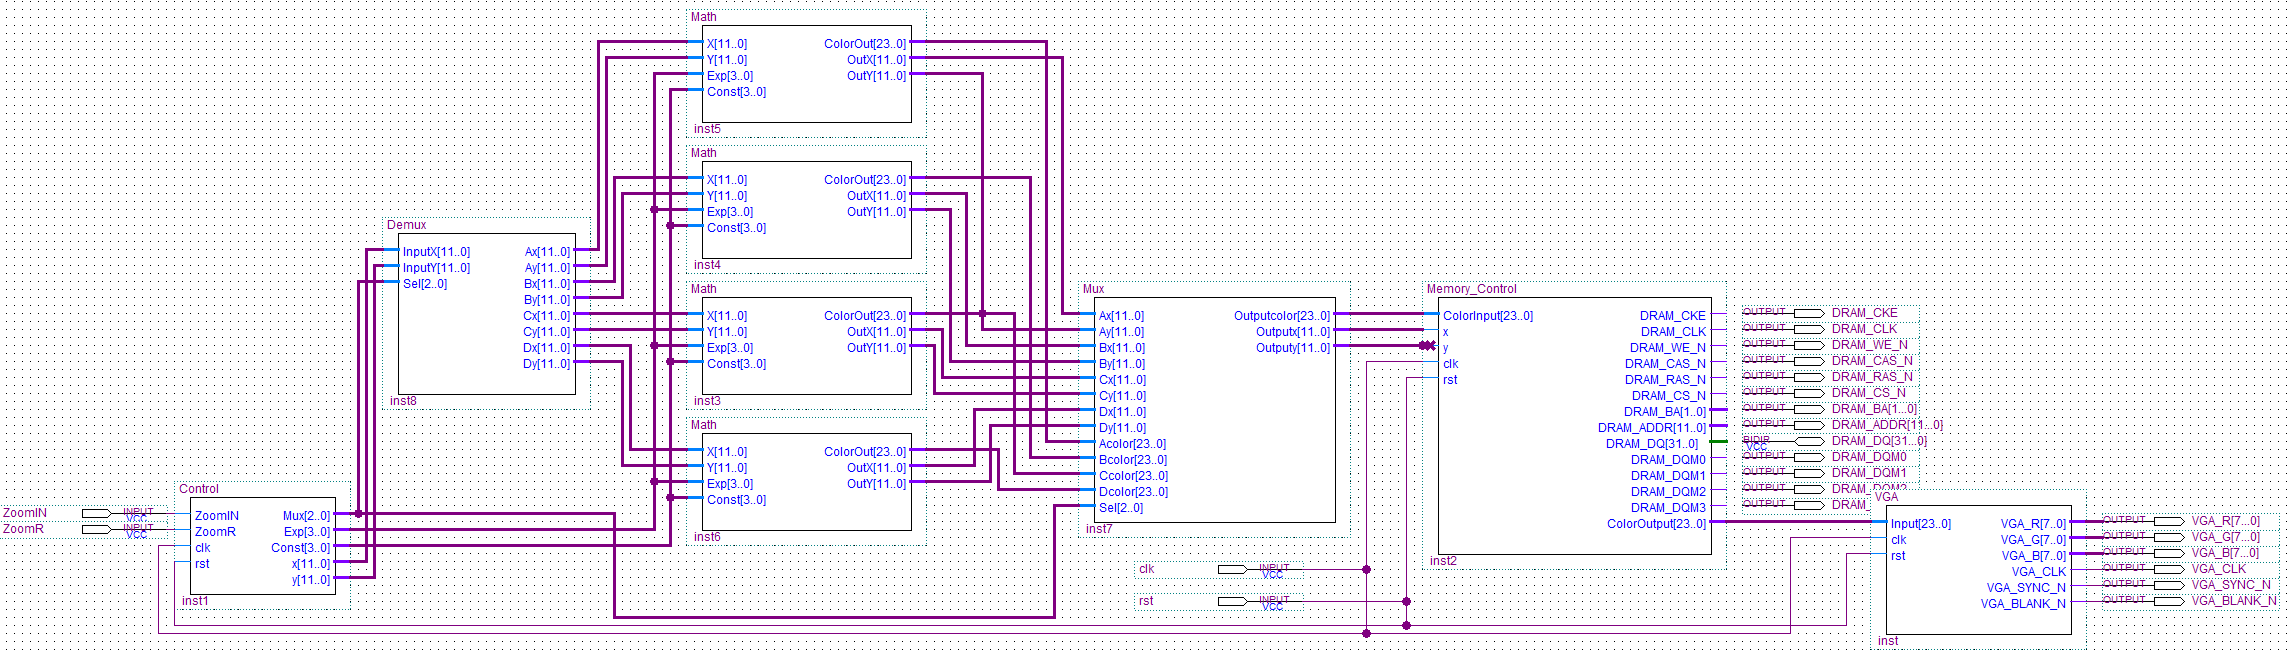
\includegraphics[width=4in]{Diagram}
\end{figure}
\end{frame}

\begin{frame}
\frametitle{Revised Design}
\begin{figure}[H]
\centering
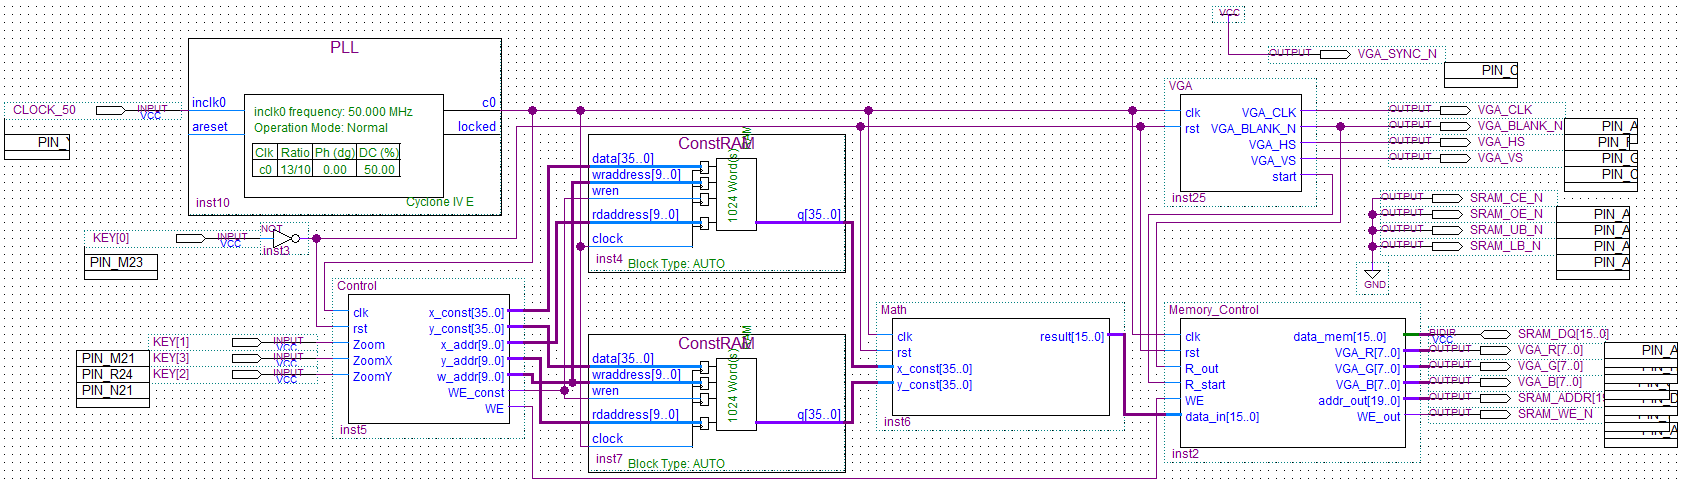
\includegraphics[width=4in]{FinalDiagram}
\end{figure}
\end{frame}

\begin{frame}
\frametitle{Considerations}
DRAM would need to run on a different clock, lots of logic needed to make it happen.
\pause
\linebreak
Parallel design requires more control signals for completion. Pipelined design does not fully use multipliers.
\pause
\linebreak
Twice the 9 bit multipliers are needed for 36 bit fixed point arithmetic than the expected 4 per multiply.
\end{frame}
\end{document}

